\documentclass[10pt]{article}

\usepackage[hmargin=0.76in,vmargin=0.62in]{geometry}
\usepackage[T1]{fontenc}
\usepackage{lmodern}
\usepackage{microtype}
\usepackage{amsmath,amssymb,amsthm,mathtools}
\usepackage{enumitem}
\usepackage{titlesec}
\usepackage{xcolor}
\usepackage{tikz}
\usetikzlibrary{arrows.meta}
\usepackage[hidelinks]{hyperref}

\setlength{\parindent}{0pt}
\setlength{\parskip}{2pt}
\setlength{\emergencystretch}{3em}
\setlength{\abovedisplayskip}{5pt}
\setlength{\belowdisplayskip}{5pt}
\setlength{\abovedisplayshortskip}{3pt}
\setlength{\belowdisplayshortskip}{3pt}
\setlist[enumerate]{leftmargin=1.45em,itemsep=1pt,topsep=2pt}
\titlespacing*{\section}{0pt}{7pt}{2pt}
\titlespacing*{\subsection}{0pt}{5pt}{1pt}
\titleformat{\section}{\large\bfseries}{}{0pt}{}
\titleformat{\subsection}{\normalsize\bfseries}{}{0pt}{}

\newtheorem{proposition}{Proposition}
\theoremstyle{definition}
\newtheorem{definition}{Definition}
\newtheorem{corollary}{Corollary}
\newcommand{\dd}{\mathrm d}

\definecolor{oldblue}{HTML}{2B5C88}
\definecolor{newred}{HTML}{B1433E}
\definecolor{midgray}{HTML}{666666}

\begin{document}

\begin{center}
{\LARGE\bfseries Housing Reallocation and Demographic Transitions}\par
\vspace{2pt}
{\large A two-generation model}\par
\end{center}

\section{Environment}

\textbf{Agents.} Time is discrete and one period is one generation. At date
$t$, the economy contains $Y_t$ young households and $O_t$ old households. A
young household has income $y_i$ and liquid wealth $b_i$, drawn from a fixed
type distribution $F$. A young renter becomes an old renter, a young owner
becomes an old incumbent, and every old household exits at the end of the
period.

\textbf{Preferences.} A young household values adult consumption $c$, space
net of children's needs, and completed fertility:
\begin{equation}
 u_t^Y(c,h,n)=\log c+\alpha\log(h-\kappa n)+\vartheta_t\log n.
 \label{eq:young_utility}
\end{equation}
Each child uses $\chi>0$ units of goods and $\kappa>0$ units of space. An old
household values consumption, retained housing, and the estate delivered at
death:
\begin{equation}
 u^O(c^O,h^O,e)=\log c^O+\gamma\log h^O+\omega_B\log e.
 \label{eq:old_utility}
\end{equation}
All choices lie in the log domain:
$c,n,h-\kappa n,c^O,h^O,e>0$. A competitive financial sector trades a claim
delivering one unit of next-period goods at price $q$, finances mortgages at
the corresponding gross return, and buys stepped-up estate housing at the
market price.

\textbf{Housing and financial markets.} A fixed stock $\bar H$ produces one
unit of housing services per unit and period. Renters can occupy at most
$\bar h^R$, while owners can occupy at most $\bar h^O>\bar h^R$. The asset
price is $P_t$, one-period-ahead goods have price $q\in(0,1)$, and
$R=q^{-1}$. Competitive housing intermediaries imply the user-cost relation:
\begin{equation}
 r_t=(1+\tau^p)P_t-qP_{t+1},
 \label{eq:user_cost}
\end{equation}
where $\tau^pP_t$ is the recurring property tax per unit.

\textbf{Ownership and taxation.} A buyer finances the share $\phi$ of the
purchase with a one-period mortgage and posts $(1-\phi)P_th$ at closing. The
mortgage advance is $\phi P_th$ and its next-period repayment is
$R\phi P_th$. Selling a unit realizes the capital-gains tax
\begin{equation}
 \ell_t=\tau^g[P_t-P_{t-1}]_+,
 \label{eq:gains_tax}
\end{equation}
while a unit retained until death enters the estate with stepped-up basis. The
tax is zero whenever the real asset price is constant. Only household sales are
taxable events; stepped-up estate liquidations are exempt, and intermediaries
trade at $P_t$ with basis marked to market.
Retained housing is occupied by the incumbent: households do not operate as
landlords, and rental services are supplied only by intermediaries. The policy
parameters $\tau^p$ and $\tau^g$ are constant. These cash flows give two
tenure-specific costs. Buying a unit, paying its
property tax, and selling it next period costs:
\begin{equation}
 r_t^O=(1+\tau^p)P_t-q(P_{t+1}-\ell_{t+1})
 =r_t+q\ell_{t+1}.
 \label{eq:owner_user_cost}
\end{equation}
For an old incumbent, retaining a unit rather than selling it, paying the
property tax, and placing its next-period value in the estate costs:
\begin{equation}
 r_t^I=(P_t-\ell_t)+\tau^pP_t-qP_{t+1}=r_t-\ell_t.
 \label{eq:incumbent_user_cost}
\end{equation}
Thus the buyer anticipates the future tax, while the incumbent avoids the
current tax by retaining the house.

\textbf{Demography.} Each child generates $\nu>0$ future young households
after survival and household formation. The children of a household affect
future cohort size but do not inherit that household's individual state.

\section{Household problems}

\subsection{Old households}

An old incumbent enters with net financial wealth $a$ and a house $H$. In
current-value terms, selling the entire house produces $(P_t-\ell_t)H$;
retained housing costs $r_t-\ell_t$ by
equation~\eqref{eq:incumbent_user_cost}. Her problem is therefore:
\begin{align}
 V_t^O(a,H)=\max_{c^O,h^O,e}\;&u^O(c^O,h^O,e)
 \label{eq:old_owner_problem}\\
 \text{subject to}\quad
 &c^O+q e+(r_t-\ell_t)h^O
 =a+(P_t-\ell_t)H+T_t,\qquad 0<h^O\leq H,
 \qquad e\geq P_{t+1}h^O.\nonumber
\end{align}
The estate includes the next-period value of retained housing. When its
composition constraint and $h^O\leq H$ are slack and $r_t>\ell_t$, the
incumbent's marginal value of retained space is:
\begin{equation}
 \frac{u_h^O}{u_c^O}=\frac{\gamma c_t^O}{h_t^O}=r_t-\ell_t.
 \label{eq:old_marginal_value}
\end{equation}
An old renter has no house and no realization. She maximizes
$u^O(c^O,h^O,e)$ subject to
$c^O+qe+r_th^O=a+T_t$, $0<h^O\leq\bar h^R$, and $e>0$.

\subsection{Young households}

Conditional on renting, a young household chooses current consumption,
housing, fertility, and saving:
\begin{align}
 W_t^R(i)=\max_{c,h,n,a'}\;&u_t^Y(c,h,n)+\beta V_{t+1}^R(Ra')
 \label{eq:young_renter_problem}\\
 \text{subject to}\quad
 &c+\chi n+a'+r_th=y_i+b_i+T_t,\qquad
 0<h\leq\bar h^R,\quad a'\geq0.\nonumber
\end{align}
Conditional on owning, the same household purchases $h$ units, posts the down
payment at the beginning of the period, and repays the mortgage when old:
\begin{align}
 W_t^O(i)=\max_{c,h,n,a'}\;&u_t^Y(c,h,n)
 +\beta V_{t+1}^O(a_{t+1},h)
 \label{eq:young_owner_problem}\\
 \text{subject to}\quad
 &c+\chi n+a'+[(1-\phi)+\tau^p]P_th=y_i+b_i+T_t,\nonumber\\
 &a_{t+1}=Ra'-R\phi P_th,\qquad
 (1-\phi)P_th\leq b_i,\nonumber\\
 &0<h\leq\bar h^O,\qquad a'\geq0.\nonumber
\end{align}
Income received after closing can finance consumption and saving but cannot be
pledged for the down payment. The household chooses the tenure with the higher
value.

Suppose saving is interior and the future old retention limit is slack. For
$m\in\{R,O\}$, let
$\lambda_t^m$ be the multiplier on the young budget, $\mu_t$ the multiplier on
the owner's down-payment constraint, and $\eta_t^m$ the multiplier on the
tenure-specific size limit. The access values in current goods are:
\begin{equation}
 \zeta_t^R=\frac{\eta_t^R}{\lambda_t^R},\qquad
 \zeta_t^O=
 \underbrace{\frac{\mu_t}{\lambda_t^O}(1-\phi)P_t}_{\zeta_t^{O,F}}
 +\underbrace{\frac{\eta_t^O}{\lambda_t^O}}_{\zeta_t^{O,S}}.
 \label{eq:access_values}
\end{equation}
Using the saving Euler equation and the old value-function envelopes, the
housing conditions reduce to:
\begin{equation}
 \frac{\alpha c_t^m}{h_t^m-\kappa n_t^m}
 =r_t^m+\zeta_t^m,\qquad
 r_t^R=r_t,\qquad r_t^O=r_t+q\ell_{t+1}.
 \label{eq:housing_foc}
\end{equation}
The ownership expression follows from the purchase, mortgage, property-tax,
and resale cash flows in equation~\eqref{eq:young_owner_problem}.
Equivalently, the access value is the household's marginal valuation above its
tenure-specific user cost:
\begin{equation}
 \zeta_t^m=
 \frac{\alpha c_t^m}{h_t^m-\kappa n_t^m}-r_t^m.
 \label{eq:observable_access_value}
\end{equation}
Thus the wedge is expressible from the household's bundle and prices, not only
from multipliers.

The fertility condition prices the goods and space required by a marginal
child:
\begin{equation}
 \frac{\vartheta_t c_t^m}{n_t^m}
 =\chi+\kappa(r_t^m+\zeta_t^m).
 \label{eq:fertility_foc}
\end{equation}
A housing constraint raises the household's shadow price of a child by
$\kappa\zeta_t^m$.

\section{Steady states and transition}

Let $G_t$ denote the normalized distribution of old net financial wealth,
inherited housing, and tenure. It is the pushforward of $F$ under the preceding
young policies:
\begin{equation}
 G_{t+1}=\operatorname{Law}_{i\sim F}\!\left(
 Ra_t'(i)-\mathbf 1\{m_t(i)=O\}R\phi P_th_t(i),
 \mathbf 1\{m_t(i)=O\}h_t(i),m_t(i)\right).
 \label{eq:old_distribution}
\end{equation}
Let $\bar n_t$, $\bar h_t^Y$, and $\bar h_t^O$ denote fertility and housing
averaged over $F$ and $G_t$, respectively.
Let $\bar s_t^O$ denote housing sold by the average old household, assigning
zero sales to old renters. Cohort sizes and the housing stock obey:
\begin{equation}
 Y_{t+1}=\nu\bar n_tY_t,\qquad O_{t+1}=Y_t,
 \qquad Y_t\bar h_t^Y+O_t\bar h_t^O=\bar H.
 \label{eq:cohort_and_housing}
\end{equation}
Fertility determines the next young cohort, while current young and old
households compete for the fixed housing stock.

The government rebates property- and capital-gains-tax receipts equally across
living households:
\begin{equation}
 (Y_t+O_t)T_t
 =\tau^pP_t\bar H+\ell_t O_t\bar s_t^O.
 \label{eq:government_budget}
\end{equation}
The taxes remain private wedges, while their revenue stays within the household
sector.

For a constant fertility preference $\vartheta$, let
$\mathcal N(P,T;\vartheta)$, $\mathcal H^Y(P,T;\vartheta)$, and
$\mathcal H^O(P,T;\vartheta)$ denote stationary fertility and housing choices
aggregated across household types.

\begin{definition}[Positive steady state]
A positive steady state is a constant equilibrium with $Y^*=O^*>0$, a constant
asset price and transfer, and stationary household policies and distributions.
Its aggregate conditions are:
\begin{align}
 1&=\nu\mathcal N(P^*,T^*;\vartheta),
 \label{eq:ss_replacement}\\
 \bar H&=Y^*\big[\mathcal H^Y(P^*,T^*;\vartheta)+
 \mathcal H^O(P^*,T^*;\vartheta)\big],
 \label{eq:ss_housing}\\
 2Y^*T^*&=\tau^pP^*\bar H.
 \label{eq:ss_government}
\end{align}
The old-state distribution is stationary: $G^*=\Gamma(P^*,T^*;\vartheta)$.
\end{definition}
The replacement condition determines whether a positive stationary population
is feasible; housing clearing and the balanced rebate jointly characterize its
price, transfer, and scale. Because $P_t=P_{t-1}$, equation
\eqref{eq:gains_tax} gives $\ell^*=0$ in every steady state.
Equation~\eqref{eq:ss_replacement} also implies that every positive steady state
has the same average fertility, $\mathcal N=1/\nu$. A permanent preference
change can alter the stationary price, transfer, population scale, and household
policies. Conditional on convergence to a positive steady state, demographic
stationarity nevertheless requires average fertility to equal $1/\nu$.

Consider two fertility preferences, $\vartheta^0$ and $\vartheta^1$, for which
the steady-state conditions admit positive equilibria $\mathcal E^0$ and
$\mathcal E^1$. At date zero the preference changes permanently:
\begin{equation}
 \vartheta_t=
 \begin{cases}
  \vartheta^0,&t<0,\\
  \vartheta^1,&t\geq0.
 \end{cases}
 \label{eq:preference_shock}
\end{equation}
The shock changes current choices immediately and future cohort sizes through
equation~\eqref{eq:cohort_and_housing}.

\begin{definition}[Transition equilibrium]
Given the initial steady state $\mathcal E^0$, a perfect-foresight transition
equilibrium is a sequence of prices, transfers, household policies,
old-household distributions, and cohort masses such that all old and young
households solve the problems above; the old distribution is generated by the
preceding young choices; housing clears and the government budget balances at
every date; equation~\eqref{eq:user_cost} prices the housing asset;
equation~\eqref{eq:cohort_and_housing} advances the cohorts; the policy
parameters $(\tau^p,\tau^g)$ remain fixed; $P_{-1}=P^0$,
$Y_0=O_0=Y^0$, $G_0=G^0$, and the date-zero old enter with the state inherited from
$\mathcal E^0$; and the sequence converges to $\mathcal E^1$.
\end{definition}
The date-zero cohort masses, old states, and tax basis $P_{-1}$ are inherited;
$P_0$, $T_0$, and household choices are equilibrium objects at impact. Capital
gains arise only on dates with $P_t>P_{t-1}$ and vanish at both stationary
endpoints. The definition imposes convergence but no monotonicity or sign on
the transition path.

\section{Intergenerational housing allocation}

Consider an old incumbent whose retention and estate-composition constraints
are slack with $r_t>\ell_t$, and a young owner whose down-payment constraint
binds while the owner-size limit and next-period old constraints are slack.
Their marginal values of current housing services are:
\begin{equation}
 MV_{it}^Y=r_t+q\ell_{t+1}+\zeta_{it}^{O,F},
 \qquad
 MV_{jt}^O=r_t-\ell_t.
 \label{eq:two_marginal_values}
\end{equation}
The market component cancels when a unit is transferred between them.

\begin{definition}[Local compensated housing test]
At a positive steady state, an allocation passes the local compensated housing
test if no infinitesimal transfer of title and occupancy from an old incumbent
to a current young owner, together with balanced goods transfers between the
two households, can leave both weakly better off and one strictly better off.
The comparison holds prices, fertility, cohort masses, tenure labels, and
constraint active sets fixed. The current young household's lifetime utility
includes its own old age; no unborn household enters the comparison.
\end{definition}

\begin{proposition}[Steady-state intergenerational reallocation]
Suppose an institution can convey a marginal unit of existing housing from an
old incumbent $j$ to a financing-constrained young owner $i$, finance the
transaction within the two-household coalition, and incur real cost $K_{ij}$
per unit. At either positive steady state, the goods-equivalent surplus is:
\begin{equation}
 \mathcal S_{ij}^*=\zeta_i^{O,F}-K_{ij}.
 \label{eq:ss_reallocation_surplus}
\end{equation}
The steady-state allocation fails the local compensated housing test whenever
$\mathcal S_{ij}^*>0$.
\end{proposition}

\begin{proof}
At a steady state, $\ell_t=\ell_{t+1}=0$. Equation
\eqref{eq:two_marginal_values} therefore values an additional unit at
$r^*+\zeta_i^{O,F}$ for the young owner and at $r^*$ for the old incumbent.
Convey $\dd h$ units of title and occupancy from $j$ to $i$, relaxing the
buyer's down-payment constraint with a pledgeable bridge
$L=(1-\phi)P^*\dd h$ at closing and repayment $RL$ next period. The advance
raises the young household's Lagrangian by $(\lambda_i+\mu_i)L$, while the
repayment lowers it by $\beta V_{a,i,t+1}^ORL$. The saving Euler equation
$\lambda_i=\beta RV_{a,i,t+1}^O$ gives
\begin{equation*}
 (\lambda_i+\mu_i)L-\beta V_{a,i,t+1}^ORL
 =\mu_iL=\lambda_i\zeta_i^{O,F}\dd h.
\end{equation*}
The unit returns to
the competitive market at $t+1$, so later housing allocations are unchanged.
The old incumbent sells the same marginal unit. At an interior retention
choice, the extra sale proceeds and the change in estate resources compensate
her marginal loss of housing services. No realization tax is due at a constant
price. Paying the real implementation cost therefore leaves
$(\zeta_i^{O,F}-K_{ij})\dd h$ goods. If this amount is positive, it can be
divided so that both households are weakly better off and one is strictly
better off.
\end{proof}

\begin{corollary}[Transition valuation gap]
At any date along the transition, the difference between the two households'
marginal valuations is:
\begin{equation}
 MV_{it}^Y-MV_{jt}^O
 =\zeta_{it}^{O,F}+q\ell_{t+1}+\ell_t.
 \label{eq:transition_valuation_gap}
\end{equation}
Capital gains therefore widen the private allocation gap when the incumbent
realizes appreciation at $t$ or the buyer anticipates appreciation at $t+1$;
the gap reduces to $\zeta_i^{O,F}$ at either stationary endpoint.
\end{corollary}
The corollary does not rank whole transition paths: doing so would require a
rule for distributing tax rebates across dates and cohorts.

\begin{figure}[b!]
\centering
\small
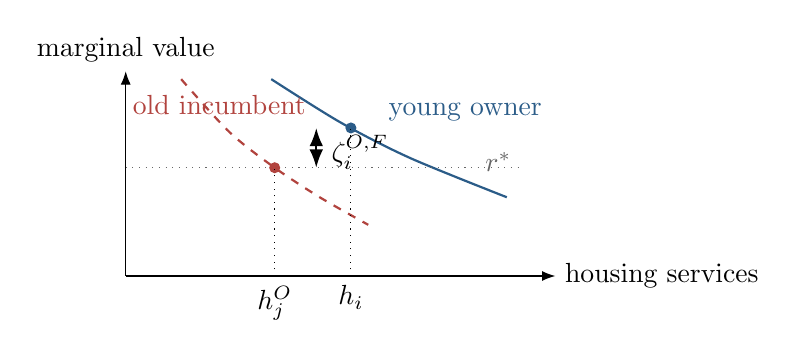
\begin{tikzpicture}[x=0.88cm,y=0.50cm,>=Latex]
  \draw[->] (0,0) -- (6.2,0) node[right] {housing services};
  \draw[->] (0,0) -- (0,5.2) node[above] {marginal value};
  \draw[oldblue,thick] plot[smooth] coordinates
    {(2.1,5.0) (3.1,3.9) (4.1,3.0) (5.5,2.0)};
  \draw[newred,thick,dashed] plot[smooth] coordinates
    {(0.8,5.0) (1.5,3.65) (2.15,2.75) (2.8,2.0) (3.5,1.3)};
  \draw[dotted,midgray] (0,2.75) -- (5.7,2.75);
  \node[right,midgray] at (5.05,2.9) {$r^*$};
  \fill[oldblue] (3.25,3.76) circle (2pt);
  \fill[newred] (2.15,2.75) circle (2pt);
  \draw[dotted] (3.25,0) -- (3.25,3.76);
  \draw[dotted] (2.15,0) -- (2.15,2.75);
  \draw[<->,thick] (2.75,2.75) -- (2.75,3.76);
  \node[right] at (2.83,3.15) {$\zeta_i^{O,F}$};
  \node[oldblue] at (4.9,4.15) {young owner};
  \node[newred] at (1.35,4.35) {old incumbent};
  \node[below] at (3.25,0) {$h_i$};
  \node[below] at (2.15,0) {$h_j^O$};
\end{tikzpicture}
\caption{At a positive steady state, the financing wedge raises the constrained
young owner's marginal value above the unconstrained incumbent's common user
cost. The gap is gross of real implementation cost.}
\label{fig:reallocation}
\end{figure}

The reallocation result and the fertility response are distinct. Let
$A=1+\gamma+\omega_B$ and $k=\beta A$. With interior saving and old choices,
substituting the old allocation and the saving Euler equation into either young
problem gives the lifetime resource identity:
\begin{equation}
 (1+k)c+\chi n+r_t^m h=\mathcal W_t,
 \qquad
 \mathcal W_t=y_i+b_i+T_t+qT_{t+1}.
 \label{eq:lifetime_budget}
\end{equation}
Suppose an access constraint fixes the household's housing at $\widehat h$ while
fertility remains interior. Holding $\mathcal W_t$ and prices fixed, implicitly
differentiating the fertility condition yields:
\begin{equation}
 \frac{\dd n}{\dd \widehat h}
 =\frac{
 \dfrac{\alpha\kappa}{(\widehat h-\kappa n)^2}
 -\dfrac{(1+k)\chi r_t^m}
 {(\mathcal W_t-r_t^m\widehat h-\chi n)^2}}
 {\dfrac{\vartheta_t}{n^2}
 +\dfrac{(1+k)\chi^2}
 {(\mathcal W_t-r_t^m\widehat h-\chi n)^2}
 +\dfrac{\alpha\kappa^2}{(\widehat h-\kappa n)^2}}.
 \label{eq:fertility_cap_derivative}
\end{equation}
The denominator is positive. The first term in the numerator is the value of
additional family space; the second is the consumption cost of occupying more
housing. Equation
\eqref{eq:housing_foc} implies
$[\mathcal W_t-r_t^m\widehat h-\chi n]/[\widehat h-\kappa n]
=(1+k)(r_t^m+\zeta_t^m)/\alpha$. For $r_t^m>0$, the exact sign condition is:
\begin{equation}
 \frac{\dd n}{\dd\widehat h}\geq0
 \quad\Longleftrightarrow\quad
 \chi\leq
 \frac{(1+k)\kappa(r_t^m+\zeta_t^m)^2}{\alpha r_t^m}.
 \label{eq:fertility_exact_condition}
\end{equation}
Since $\zeta_t^m\geq0$, a simpler sufficient condition is:
\begin{equation}
 \chi\leq\frac{(1+k)\kappa r_t^m}{\alpha}.
 \label{eq:fertility_sufficient_condition}
\end{equation}
Under this condition, relaxing access and permitting the household to purchase
more housing at its market user cost raises its fertility. Separately,
Proposition~1 implies that a marginal housing transfer passes the local
compensated test when $K_{ij}<\zeta_i^{O,F}$. The two conditions can hold
simultaneously, but they are distinct results.
General-equilibrium prices, rebates, and cohort sizes then propagate that
response through
equations~\eqref{eq:cohort_and_housing}--\eqref{eq:government_budget}.

\end{document}
